\documentclass[sigplan]{acmart}
\usepackage{subcaption}
\usepackage{caption}
\usepackage{array}
\usepackage{multirow}
%%
%% \BibTeX command to typeset BibTeX logo in the docs
\AtBeginDocument{%
  \providecommand\BibTeX{{%
    \normalfont B\kern-0.5em{\scshape i\kern-0.25em b}\kern-0.8em\TeX}}}

\setcopyright{none}
\copyrightyear{}
\acmYear{}
\acmDOI{}

\acmConference[]{Introduction to Research}{December 2021}{Lisbon}
\acmBooktitle{}
\acmPrice{}
\acmISBN{}


%% end of the preamble, start of the body of the document source.
\begin{document}

%%
%% The "title" command has an optional parameter,
%% allowing the author to define a "short title" to be used in page headers.
\title{Desenvolvimento de uma Aplicação em Orientação a Objetos}

%%
%% The "author" command and its associated commands are used to define
%% the authors and their affiliations.
%% Of note is the shared affiliation of the first two authors, and the
%% "authornote" and "authornotemark" commands
%% used to denote shared contribution to the research.

\author{Pedro Miguel Ferreira Tavares Carrega - 49480}
\affiliation{
 \institution{ Estudo Orientado em Engenharia Informática \\ Mestrado em Engenharia Informática \\ Faculdade de Ciências, Universidade de Lisboa}
 }
\email{fc49480@alunos.fc.ul.pt}


\renewcommand{\shortauthors}{Pedro Miguel Ferreira Tavares Carrega - 49480}

%%
%% The abstract is a short summary of the work to be presented in the
%% article.
\begin{abstract}
  Este relatório foi desenvolvido com o propósito de descrever o ambito do tema de tese a ser entregue no fim deste ano lectivo e detalhar o trabalho até agora realizado. 
\end{abstract}


%%
%% Keywords. The author(s) should pick words that accurately describe
%% the work being presented. Separate the keywords with commas.
\keywords{ARTSOFT, ERP, OOP, C++, Segurança Social}


%%
%% This command processes the author and affiliation and title
%% information and builds the first part of the formatted document.
\maketitle

\section{Introduction}

Here you should motivate your work. 

What is the context? \\ %introduzir ARTSOFT

What is the problem? \\ %o k é pretendido

Why is it important? \\ %o cliente quer e poupar TEMPO aos utilizadores

What data and methods are you thinking about using to tackle it? \\ %prob no data. methods no good idea how to explain

How is this document organised? \\

\section{Background} \label{sec:background}

\subsection{Ferramentas Utilizadas}

\subsubsection{ARTSOFT}



\subsubsection{TortoiseSVN}

O TortoiseSVN é um cliente \textit{open source} para a aplicação Apache Subversion oferecendo uma interface gráfica, um submenu de contexto no explorador do windows e acesso rápido a todos os comandos oferecidos pelo Subversion. Subversion é uma aplicação de controlo de versões que corre num servidor centralizado. Uma arquitetura centralizada oferece várias vantagens em comparação com uma arquitetura distribuída: O repositório encontra-se hospedado num servidor central, retirando a necessidade de clonar o repositório na sua totalidade. Isto também permite a atualização somente dos ficheiros locais. Ambos estes fatores levam a uma carga inferior da rede, contudo também implica se o servidor central se encontrar em baixo também se encontra o serviço. Subversion também permite a definição de restrição de acessos e o bloqueio de escrita simultânea de ficheiros, impedido o merge de binários.

\subsubsection{Jenkins}

\textit{DevOps} é um conjunto de filosofias e práticas que promovem o desenvolvimento e lançamento de aplicações com maior rapidez e qualidade. Duas das práticas mais relevantes são \textit{Continuous Integration} e \textit{Continuous Delivery}. \textit{Continuous Integration} é uma prática aonde programadores integram, com regularidade, código desenvolvido para um repositório central sendo automaticamente compilado e efetuados testes sobre o mesmo. Este depois é automaticamente preparado para lançamento, sendo esta a base de \textit{Continuous Delivery}. Com o objetivo de promover estas práticas a empresa ARTSOFT usa a ferramenta Jenkins - um servidor de automação \textit{open source} que corre em \textit{servlet containers} facilitando \textit{Continuous Integration} e \textit{Continuous Delivery} através de \textit{pipelines} para automizar a compilação de binários através da definição de um conjunto de processos que permitem às pipelines compilar, construir e lançar automaticamente o código produzido.

%adicionar imagem de 1 pipeline

\subsection{Eventos}

Um evento é um registo interno que é criado na aplicação ARTSOFT sempre que ocorra um acontecimento. Dentro da empresa ARTSOFT é utilizado para efetuar o registo de vários tipos de acontecimentos sendo os mais comuns os eventos de reporte de bug e eventos de roadmap. Roadmap são eventos que envolvem o desenvolvimento de funcionalidades para futuras versões do ARTSOFT. Eventos que reportam bugs no funcionamento da aplicação ARTSOFT, estes eventos podem ser criados devido a reportes internos ou por clientes da aplicação ARTSOFT. Um evento de bug ao ser criado é enviado para a entrada do Departamento de Programação (DRP), aí o mesmo é atribuído a um membro da equipa. O programador responsável pelo evento ao concluir o seu trabalho transfere o evento para a Unidade de Qualidade de Software (UQS). A equipa de testes vai testar o evento, confirmando se o mesmo se encontra resolvido. Caso o evento se encontre resolvido é assinalado como tal e é passado para a saída do DPR, senão o evento é passado de volta para o programador responsável pelo evento.

\begin{figure}[htbp]
	\centerline{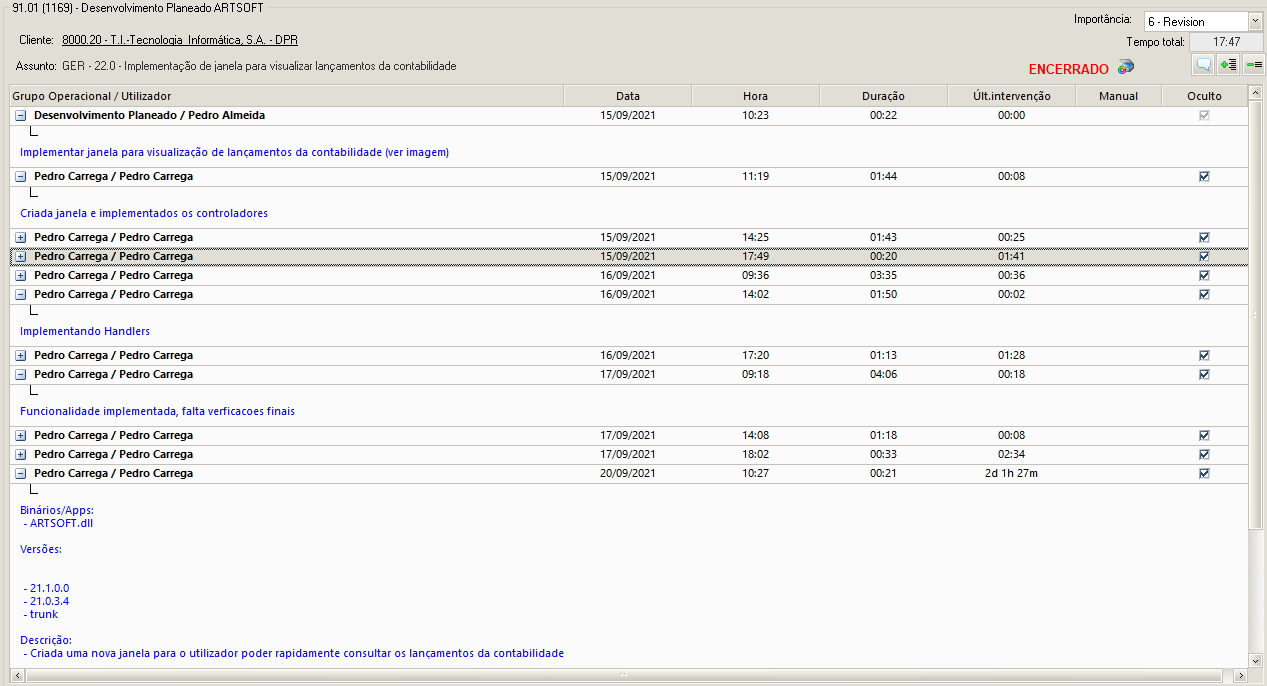
\includegraphics[width=\linewidth]{figures/evento_formacao.png}}
	\caption{Example of an event.}
	\label{fig1}
\end{figure}

\subsection{Formação}

Os primeiros três meses da minha tese foram dedicados à minha formação. O primeiro dia foi dedicado a ensinar-me os conceitos básicos do funcionamento da aplicação ARTSOFT, o funcionamento das ferramentas utilizadas para o controlo de versões e como funciona o fluxo de um evento. O restante da minha primeira semana foi dispendido a tratar de um evento de tipo roadmap, evento que foi criado somente com o propósito de formação, que me deu contacto com tudo que iria necessitar para efetuar desenvolvimento na aplicação ARTSOFT. O evento pedia a criação de uma interface que permitisse a visualização de entradas dado um de três tipos de entradas: Diário, Documento, Conta. Os três tipos de entradas requerem o número da entrada a consultar, sendo possível fornecer diferentes tipos consoante o tipo de entrada para filtrar os resultados. O diário é possível limitar ao mês que se pretende consultar enquanto que o documento é possível filtrar por tipo de documento. 

\subsubsection{Diário}

\subsubsection{Documento}

\subsubsection{Conta}

 Após a entrega desta nova funcionalidade foi me atribuído regularmente diferentes eventos até o prazo que se inicializou o desenvolvimento na nova versão do ARTSOFT.

\section{Related Work} \label{sec:relatedwork}

This is the time to do a literature review! \\

What is the state of the art on the topic you are working? \\

Previous work with same data, similar work with other data, ... \\

Problems tackled, data science approaches used, pros and cons, ... \\ 


Example of a reference\cite{subversion}.

\section{Data \{if necessary\} } \label{sec:data}

Creio que não tenho data.

Here you should describe your data in as much detail as possible. \\ 

You can describe raw data and any pre-processing need for your work. \\

You can have a section on exploratory data analysis. \\

\section{Methods} \label{sec:methods}

Here you should describe in as much details as possible the problem and your plan to tackle it. \\

What are the methods you are planning to use, or already started to use, to tackle your problem. \\

This should be based on related word, your understanding of the problem and eventually preliminary exploratory data analysis or preliminary results.

\subsection{Problema} %alterar o nome desta seccao

\subsection{Redação da Especificação de Requisitos}

\subsection{Sprints}

\subsection{Testes}

\section{Preliminary Results (Optional)} \label{sec:preliminaryresults}

Se conseguir acesso ao ambiente de qualidade antes da entrega (prob not).

Here you can include preliminary results if you already have them.

\section{Forthcoming Work} \label{sec:forthcomingwork}

%Here you should write the conclusion of the preliminary work and the goals for the remaining period.

O passo seguinte a realizar no projeto será a realização de uma reunião para apresentar e aprovar a especificação de requisitos. Dada a aprovação, serão definidos vários SPRINTS quinzenais com diferentes objetivos vão ser implementadas as interfaces gráficas e requisitos descritos na especificação. Uma vez implementadas, irá ser utilizado o ambiente de qualidade para realizar testes de forma a confirmar o correto comportamento das funcionalidades implementadas. Estas novas funcionalidades irão ser incluídas na nova versão da aplicação ARTSOFT, aonde será realizado tratamento de bugs que surgam nas funcionalidades implementadas.

%%
%% The next two lines define the bibliography style to be used, and
%% the bibliography file.
\bibliographystyle{ACM-Reference-Format}
\bibliography{bib/bibliography}
\end{document}

\endinput
%%
%% End of file `sample-sigchi.tex'.
